\documentclass[tikz,border=8pt]{standalone}
\usetikzlibrary{arrows.meta}
\begin{document}
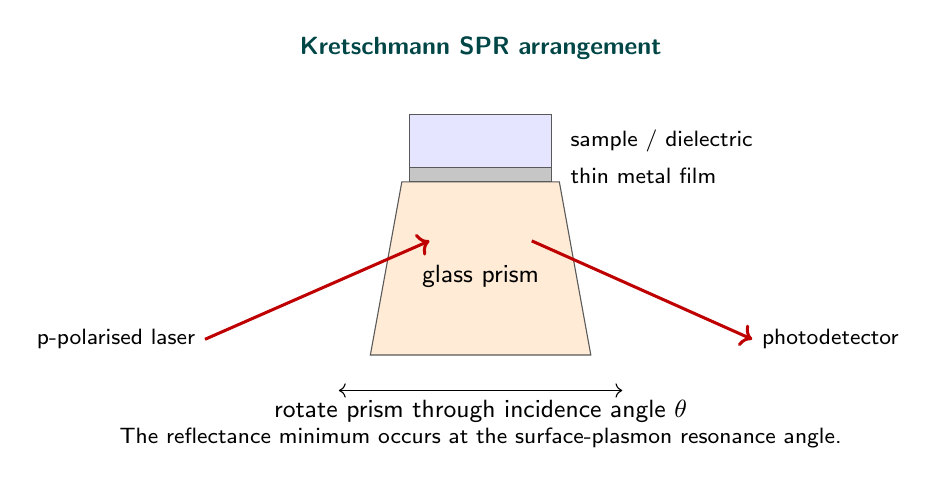
\begin{tikzpicture}[font=\sffamily\small]
\node[font=\sffamily\bfseries\small,text=teal!55!black] at (0,4.7) {Kretschmann SPR arrangement};
\draw[fill=orange!16,draw=black!65] (-1.4,.8)--(1.4,.8)--(1.0,3.0)--(-1.0,3.0)--cycle;
\node at (0,1.8) {glass prism};
\draw[fill=gray!45,draw=black!65] (-.9,3.0) rectangle (.9,3.18);
\node[right=.12cm,font=\sffamily\footnotesize] at (.9,3.08) {thin metal film};
\draw[fill=blue!10,draw=black!65] (-.9,3.18) rectangle (.9,3.85);
\node[right=.12cm,font=\sffamily\footnotesize] at (.9,3.52) {sample / dielectric};
\draw[->,red!75!black,line width=1.1pt] (-3.5,1.0)--(-.65,2.25);
\node[left,font=\sffamily\footnotesize] at (-3.5,1.0) {p-polarised laser};
\draw[->,red!75!black,line width=1.1pt] (.65,2.25)--(3.45,1.0);
\node[right,font=\sffamily\footnotesize] at (3.45,1.0) {photodetector};
\draw[<->] (-1.8,.35)--(1.8,.35) node[midway,below] {rotate prism through incidence angle $\theta$};
\node[font=\sffamily\footnotesize] at (0,-.25) {The reflectance minimum occurs at the surface-plasmon resonance angle.};
\end{tikzpicture}
\end{document}
